\setcounter{chapter}{3}
\setcounter{rq}{1}


\chapter{Android Task Corpus}
\label{ch:android-corpus}



One of the challenges for characterizing task-relevant information as well as for proposing automatic techniques to automatically identify task-relevant text is
the lack of large corpora containing
software tasks and associated artifacts originating from heterogeneous sources.
To fill this gap, this chapter contributes with the Android tasks corpus (\textbf{\acs{DS-android}}), a dataset with 300 tasks comprising Android development and originating from Stack Overflow questions
as well as from GitHub issues on a variety of Android Open-Source Systems.



This chapter main contributions are \textit{(i)} the procedures for the corpus creation, and; \textit{(ii)} the corpus itself. A well-structured corpus lays the foundation for several studies that explore relationships between software tasks, natural language artifacts, and text within these artifacts. \red{eval \& corpus summary}





\section{Motivation}
\label{cp4:motivation}


When performing a software task, a software developer does not restrict her work
solely to coding~\cite{Meyer2017}.
Rather, there are many activities that a developer undertakes to complete a software task
as when they:



\begin{itemize}
    \item refer to API documentation or Q\&A websites for API usage purposes~\cite{umarji2008archetypal, Singer1998, robillard2011field};
    \item discuss in mailing lists a possible reusable library to be incorporated into their implementation~\cite{umarji2008archetypal, Bacchelli2012}; or
    \item confirm a system's behaviour referring to past discussions in community forums or in the system's documentation~\cite{Arya2019, Lotufo2012, Singer1998}.
\end{itemize}


A common aspect to these activities is the need to work with unstructured textual data, which comprises 80\% of the overall information created and used in enterprises~\cite{Bavota2014, holzinger2013}.
Due to such prevalence, there has been a large body of studies utilizing various techniques to extract
information from this text so that it can be embedded in
tools to software developers~\cite{Bavota2014, Xu2017, Robillard2015, Lotufo2012}. For instance, Xu et al. propose to mine relevant text from Stack Overflow
to generate answers to developers' technical question~\cite{Xu2017}
while FRAPT identifies key paragraphs explaining API elements in code tutorials~\cite{Jiang2017}.
As other examples, Lotufo et al. proposed a technique to identify sentences a developer would first read when inspecting bug reports~\cite{Lotufo2012} while Nadi and Treude investigated sentences that help a developer decide whether a Stack Overflow post is relevant to her task~\cite{nadi2020}.




Although these studies provide significant contributions, the fact that information to answer a question a developer has is usually located across many artifacts~\cite{Rastkar2013t} is often overlooked.
Hence existing techniques operate in an artifact-centric basis
what can be insufficient to provide to developers all the information needed
to completely and correctly accomplish a software task as several studies suggest that developers use heterogeneous sources to put together the information needed for task completion~\cite{josyula2018, Li2013, rao2020}.




We seek to design techniques that can scale to cover different types of artifacts
so that can be integrated into developers' information-seeking activities regardless of the artifact that a developer browses/inspects.
To design such techniques, we require a corpus with heterogeneous sources that a developer
might use to locate information relevant to her task.


\section{Corpus Creation}
\label{cp4:corpus-creation}

Corpus creation consists of three main steps, namely \textit{(1)} selection of tasks, \textit{(2)} selection of artifacts, and \textit{(3)} identification of relevant text within the selected artifacts. We detail each of these steps in the following sections.









\subsection{Corpus Summary}
\textcolor{white}{force ident} % this is just for the chapter outline



Figure~\ref{fig:corpus-creation-pipeline} summarizes procedures for corpus creation.
We randomly sample a set of Android development tasks from Stack Overflow and GitHub
and use the Google search engine to find potential resources that might have
information for a task. We only consider resources highly ranked at Amazon Alexa and, for these resources, we apply state of the art techniques to detect relevant text in the artifact's content.



Overall, our corpus comprises 300 tasks evenly selected from SO and Git. 
There is a total of 262,278 sentences in 2,586 artifacts pertaining API documentation, Stack Overflow answers, Github issue discussions, and miscellaneous Web tutorials or blog posts. 



\begin{figure}
    \centering
    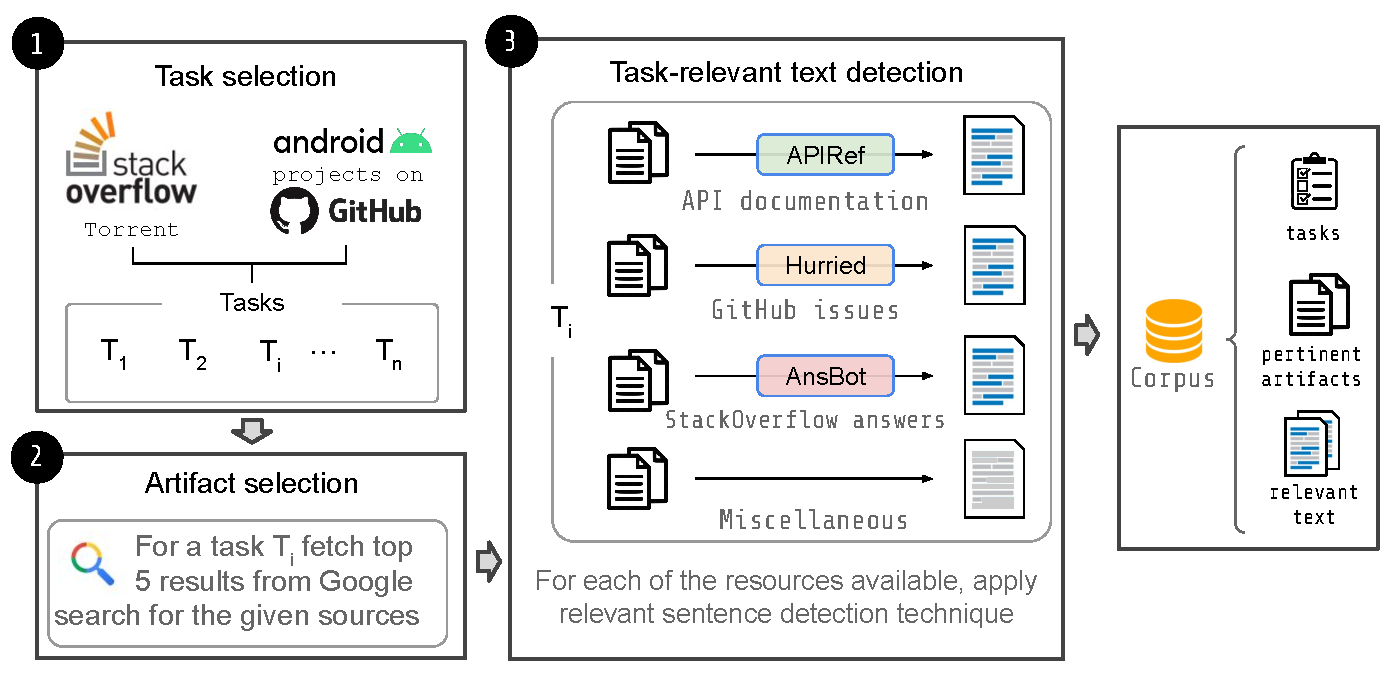
\includegraphics[width=\textwidth]{cp4/corpus-creation-pipeline}
    \caption{Summary of procedures for corpus creation}
    \label{fig:corpus-creation-pipeline}
\end{figure}




\section{Evaluation}
\label{cp4:evaluation}


To construct the \acs{DS-android} corpus, we apply a set of techniques 
to artifacts outside the ones where the techniques were originally proposed and evaluated.
For instance, \acs{AnsBot} was evaluated in a set of 100 general Java programming tasks~\cite{Xu2017} while our tasks comprise Android development.
Generalizability is a common threat emphasized in each of the techniques original studies~\cite{Xu2017, Lotufo2012, Robillard2015} and thus, there is a risk that the techniques do no apply to 
the tasks and artifacts in our corpus.




To mitigate this risk, we evaluate the accuracy of each technique on a subset of our corpus. We rely on three reference answers produced by 
experienced software developers to define \textit{golden relevant sentences} 
for a sample of 10 tasks and associated artifacts in our corpus. 
We use the golden data to evaluate and report each technique's accuracy in our corpus.
If we can show that the techniques identify relevant text with some \textit{margin of error},
future research can use our corpus for the design and comparison of techniques that identify task-relevant text automatically.




\subsection{Golden Data}


Creating golden data for the entirety of the \acs{DS-android} corpus is infeasible
since it would require asking human evaluators to inspect thousands of artifacts and more than 260,000 sentences.
Due to this reason, we restrict this evaluation to a random subset of 10 tasks in our corpus (i.e., 5 GitHub tasks and 5 Stack Overflow tasks). 
From now on, we refer to this subset as the \textbf{\acs{DS-android-small}} corpus.


For each one of the tasks in the \acs{DS-android-small} corpus, we also randomly selected 
one artifact per source type to a maximun of 4 artifacts per tasks, i.e., one API document, a Github issue discussion, one Stack Overflow answer, and a blog or Web tutorial.
% As an example, Table~\ref{tbl:googlesearch-example-git} shows the 
% artifacts an annotator inspected for the lock screen controls task.
Overall, this corpus has 2,375 sentences with an average of 64 sentences per artifact---
a size comparable to the \acs{DS-synthetic} corpus~\cite{marques2020}.
% ($\mypm$ 72)


We asked human evaluators to read the content of these artifacts and 
to mark sentences that they deemed useful and that provide information that assisted task completion.
Golden data in \acs{DS-android-small} consists of any sentence that two or more evaluators have deemed as useful for task-completion.



\subsubsection{Annotators}
\textcolor{white}{force ident} % this is just for the chapter outline

--- We recruited \red{n} graduate students with professional programming experience to produce \textit{golden} data for our tasks sample. \vspace{3mm}


\subsubsection{Annotation Procedures}

Our intention is that goldens reflect text that a experienced developer would deem as useful for task completion and that they would share with someone eager to make their \textit{first contribution} in an open-source project.


To produce such data, annotators had  at their disposal a set of randomly assigned tasks description and links to artifacts pertinent to the respective task. We asked annotators to write a short plan (250 words max~\cite{Rastkar2010}) with instructions that a newcomer could follow to successfully complete the task. 
The purpose of the plan was to ensure that annotators built enough context about the task.
While perusing artifacts, annotators also had to manually highlight sentences that they deemed useful and that provide information that assisted task completion. 


The annotation process was facilitated by an in-house tool, in the form of a Web browser plugin shown in Figure~\ref{fig:corpus-annotation-tool}. In the figure, the top-right corner panel shows the browser extension. Annotators could start an annotation session and click the highlight buttom.
This would instrument the HTML of a page and identify each sentence in a paragraph. The tool allowd annotators to hove over individual sentences and select them as relevant by clicking on the hovered text (text in orange). For example, the figure depicts that an annotator deemed the sentence
``\textit{Call {\small \texttt{ActivityOptions.setLockTaskEnabled()}} ... when starting the activity}'' as relevant for the lock mode task.


\begin{figure}
    \centering
    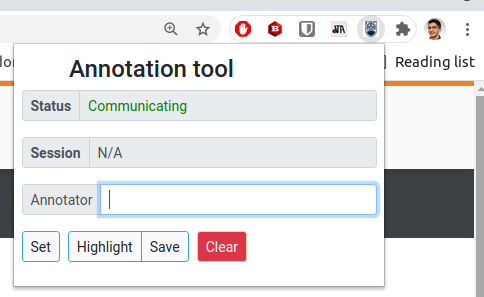
\includegraphics[width=\textwidth]{cp4/annotation-tool}
    \caption{Annotation tool and relevant sentences marked by an annotator}
    \label{fig:corpus-annotation-tool}
\end{figure}



\subsection{Evaluation Metrics}

For each task in \acs{DS-android-small}, we have a set of artifacts with task-relevant sentences identified by experienced developers. We  
compute a technique's accuracy using standard \textit{precision} and \textit{recall} metrics~\cite{Manning2009IR} by comparing the relevant text automatically identified by a technique
against the golden relevant text.



To ease interpreting evaluation metrics, Table~\ref{tbl:type-I-II-errors} show all possible evaluation outcomes. The \textit{relevant} and \textit{not-relevant} columns represent the text 
marked (or not) by the annotators. Rows represent the text automatically identified by a technique.




\begin{table}[H]
\centering    
\begin{scriptsize}
\begin{threeparttable}
\begin{tabular}{l|l|l}

\hline

\textbf{}
& \textbf{Relevant}    
& \textbf{Not-relevant} \\

\hline
\hline

\textbf{Identified as relevant} & true positive ($TP$) & false positive ($FP$) \\
\hline
\textbf{Identified as Not-relevant} & false negative ($FN$) & true negative ($TN$) \\
\hline

\end{tabular}
\end{threeparttable}
\end{scriptsize}
\caption{Result outcomes}
\label{tbl:type-I-II-errors}
\end{table}

    



For a given task $t$ and artifact $a$, precision is the ratio between the sentences identified that are marked as relevant and the total number of sentences identified, as shown in Equation~\ref{eq:cp4:precision}.


\begin{equation}
\label{eq:cp4:precision}    
    Precision(t, a) = \frac{TP}{TP + FP}
\end{equation}


Recall represents how many of all marked sentences are identified by a technique (Equation~\ref{eq:cp4:recall}).



\begin{equation}
\label{eq:cp4:recall}        
    Recall(t, a) = \frac{TP}{TP + FN}
\end{equation}

\vspace{3mm}




\subsection{Results}
\textcolor{white}{force ident} % this is just for the chapter outline


--- Discuss results \vspace{3mm}



--- Precision~\ref{tbl:ds-small-results-precision} \vspace{3mm}


--- Recall~\ref{tbl:ds-small-results-recall} \vspace{3mm}

--- Likely explanation for the results obtained.

% When interpreting results, we favor precision instead of recall.
% A false positives may contribute to a developer abandoning reading of an artifact that would otherwise provide crucial information for her task~\cite{Rastkar2010}.




\begin{table}[H]
\centering    
\begin{scriptsize}
\begin{threeparttable}
\begin{tabular}{lcccccc}

\hline


\multirow{2.5}{*}{Technique}
& \multicolumn{2}{c}{\textit{$Precision_{n=3}$}}
& \multicolumn{2}{c}{\textit{$Precision_{n=2}$}}
& \multicolumn{2}{c}{\textit{$Precision_{n=1}$}}
\\ \cmidrule(l){2-3} \cmidrule(l){4-5} \cmidrule(l){6-7} 


& \textit{mean}
& \textit{std}
& \textit{mean}
& \textit{std}
& \textit{mean}
& \textit{std}
\\


\hline
\hline

\acs{AnsBot} 
& 0.5 & 0.5 % = 3
& 0.5 & 0.5 % = 2
& 0.5 & 0.5 % = 1
\\

\acs{Krec} 
& 0.5 & 0.5 % = 3
& 0.5 & 0.5 % = 2
& 0.5 & 0.5 % = 1
\\

\acs{Hurried} 
& 0.5 & 0.5 % = 3
& 0.5 & 0.5 % = 2
& 0.5 & 0.5 % = 1
\\

\hline

\end{tabular}
\end{threeparttable}
\end{scriptsize}
\caption{Precision of each technique for the tasks of \acs{DS-android-small}}
\label{tbl:ds-small-results-precision}
\end{table}

    

% \begin{table}[H]
% \centering    
% \begin{scriptsize}
% \begin{threeparttable}
% \begin{tabular}{lcccccccccccc}

% \hline


% \multirow{2.5}{*}{Technique}
% & \multicolumn{10}{c}{\textit{Tasks}} 
% & \multicolumn{2}{c}{\textit{Precision}}
% \\  \cmidrule(l){2-11} \cmidrule(l){12-13} 



% &
% \textit{T1} & \textit{T2} & \textit{T3} & \textit{T4} & \textit{T5}
% & \textit{T6} & \textit{T7} & \textit{T8} & \textit{T9} & \textit{T10}
% & \textit{mean}
% & \textit{std}
% \\


% \hline
% \hline

% \acs{AnsBot} 
% & 0.5 & 0.5 & 0.5 & 0.5 & 0.5
% & 0.5 & 0.5 & 0.5 & 0.5 & 0.5
% & 0.5 % mean
% & 0.5 % std
% \\

% \acs{Krec} 
% & 0.5 & 0.5 & 0.5 & 0.5 & 0.5
% & 0.5 & 0.5 & 0.5 & 0.5 & 0.5
% & 0.5 % mean
% & 0.5 % std
% \\

% \acs{Hurried} 
% & 0.5 & 0.5 & 0.5 & 0.5 & 0.5
% & 0.5 & 0.5 & 0.5 & 0.5 & 0.5
% & 0.5 % mean
% & 0.5 % std
% \\

% \hline

% \end{tabular}
% \end{threeparttable}
% \end{scriptsize}
% \caption{Precision of each technique for the tasks of \acs{DS-android-small}}
% \label{tbl:ds-small-results-precision}
% \end{table}

    

\begin{table}[H]
\centering    
\begin{scriptsize}
\begin{threeparttable}
\begin{tabular}{lcccccc}

\hline


\multirow{2.5}{*}{Technique}
& \multicolumn{2}{c}{\textit{$Recall_{n=3}$}}
& \multicolumn{2}{c}{\textit{$Recall_{n=2}$}}
& \multicolumn{2}{c}{\textit{$Recall_{n=1}$}}
\\ \cmidrule(l){2-3} \cmidrule(l){4-5} \cmidrule(l){6-7} 


& \textit{mean}
& \textit{std}
& \textit{mean}
& \textit{std}
& \textit{mean}
& \textit{std}
\\


\hline
\hline

\acs{AnsBot} 
& 0.5 & 0.5 % = 3
& 0.5 & 0.5 % = 2
& 0.5 & 0.5 % = 1
\\

\acs{Krec} 
& 0.5 & 0.5 % = 3
& 0.5 & 0.5 % = 2
& 0.5 & 0.5 % = 1
\\

\acs{Hurried} 
& 0.5 & 0.5 % = 3
& 0.5 & 0.5 % = 2
& 0.5 & 0.5 % = 1
\\

\hline

\end{tabular}
\end{threeparttable}
\end{scriptsize}
\caption{Recall of each technique for the tasks of \acs{DS-android-small}}
\label{tbl:ds-small-results-recall}
\end{table}

    


\subsection{Threats to Validity}

--- Discuss threats \vspace{3mm}




% \acs{DS-android-small}

% \acs{DS-android-large}